% slides.tex
% Beamer talk: "How Autocracy Shapes the Social Sciences: Evidence from an Agent Orchestra"
% Tore Wig (UiO) -- AUTOKNOW ERC-COG. ~12-15 min workshop talk.
% Compile with XeLaTeX (3 passes) + bibtex. Reuses figures/ and tables/.

\documentclass[aspectratio=169,11pt]{beamer}

\usetheme{default}
\usecolortheme{dove}
\setbeamertemplate{navigation symbols}{}
\setbeamertemplate{itemize items}[circle]
% Footline: UiO logo (left) + frame number (right), on every slide
\setbeamertemplate{footline}{%
  \leavevmode%
  \hbox{%
    \begin{beamercolorbox}[wd=.5\paperwidth,ht=2.5ex,dp=2.5ex,leftskip=1em]{}%
      \raisebox{-1.6ex}{
\includegraphics[height=0.9cm]{UIO_logo.jpg}}%
    \end{beamercolorbox}%
    \begin{beamercolorbox}[wd=.5\paperwidth,ht=2.5ex,dp=2.5ex,rightskip=1em]{}%
      \hfill{\footnotesize\color{gray}\insertframenumber/\inserttotalframenumber}%
    \end{beamercolorbox}%
  }%
  \vskip1pt%
}

\usepackage{booktabs}
\usepackage{graphicx}
\usepackage{amsmath}
\usepackage{natbib}
\usepackage{tikz}
\usetikzlibrary{positioning, arrows.meta}

\graphicspath{{figures/}{./}}

% --- Palette (matches the manuscript pipeline figure) ---
\definecolor{agentblue}{RGB}{31,97,163}
\definecolor{gateamber}{RGB}{200,120,20}
\definecolor{milestoneteal}{RGB}{20,140,110}

\setbeamercolor{frametitle}{fg=agentblue}
\setbeamercolor{title}{fg=agentblue}
\setbeamercolor{structure}{fg=agentblue}
\setbeamerfont{frametitle}{series=\bfseries}

% --- macros (NB: avoid \fam -- it is a TeX primitive) ---
\newcommand{\key}[1]{\textcolor{agentblue}{\textbf{#1}}}
\newcommand{\good}[1]{\textcolor{milestoneteal}{#1}}
\newcommand{\warn}[1]{\textcolor{gateamber}{#1}}
\newcommand{\caveat}{{\footnotesize\color{gray}\textit{Preliminary: 21 of 25 teams done; 4 framing/embedding teams pending.}}}

\begin{document}

% ===================== 1. Title (with logos) =====================
\begin{frame}[plain]
  \vfill
  \begin{center}
    {\Large\bfseries\color{agentblue} How Autocracy Shapes the Social Sciences}\\[0.35em]
    {\large Synthesized Evidence from an Agent Orchestra}\\[1.3em]
    {\large Tore Wig}\\[0.3em]
    {\footnotesize University of Oslo \,$\cdot$\, AUTOKNOW (ERC-COG 101231399)}\\[0.5em]
    {\scriptsize\color{gray} Workshop draft, June 2026; preliminary, please do not cite}
  \end{center}
  \vfill
  \begin{center}
    
\includegraphics[height=1.0cm]{LOGO_ERC-FLAG_EU.png}\hspace{1.6cm}%
    
\includegraphics[height=1.0cm]{UIO_logo.jpg}
  \end{center}
  \vspace{0.3em}
\end{frame}

% ===================== 2. Motivation =====================
\begin{frame}{Does autocracy bend the \emph{content} of social science?}
  \begin{itemize}
    \item Autocracies are now major science producers (China $>$ US).
    \item Old claim: \key{open societies} breed good science \citep{Popper1945,kitcher2001science}.
    \item Bibliometrics shows regime effects on \key{volume} and \key{citations}
          \citep{Tayebi2025,Yang2021}.
  \end{itemize}
  \vspace{0.8em}
  \begin{block}{The gap}
    If researchers self-censor, autocracy should also shape the
    \key{contents and framing} of research, not just its quantity.
    We look at this in Social Sciences and Humanities (SSH) field. 
  \end{block}
\end{frame}

% ===================== 3. Project at a glance (NEW) =====================
\begin{frame}{The project}
  \begin{block}{Research questions}
    \begin{enumerate}
      \item Do researchers in autocracies \key{self-censor} and respond
            strategically to regime context?
      \item What are the implications for \key{social-science contents}?
    \end{enumerate}
  \end{block}
  \begin{columns}[T]
    \begin{column}{0.52\textwidth}
      \textbf{Design}
      \begin{itemize}\small
			\item An orchestra of AI-agents, to test several implications
        \item 25 \key{pre-registered} AI-agent teams
        \item One corpus: \key{2.7M} WoS SSH articles (1970--2023)
        \item Autocracy-democracy = V-Dem liberal democracy
        \item 5 sub-theory families, family-wise Bonferroni corrections
      \end{itemize}
    \end{column}
    \begin{column}{0.48\textwidth}
      \textbf{So far (21/25 teams)}
      \begin{itemize}\small
        \item \good{Essentially no signal of self-censorship theory}
        \item 0 of 21 significant
        \item Method: an \key{agent-orchestra} many-analysts design
      \end{itemize}
    \end{column}
  \end{columns}
  \vspace{0.4em}
  \centering \caveat
\end{frame}

% ===================== 4. Theory =====================
\begin{frame}{Theory: strategic self-censorship}
  \small
  \textbf{Researchers and their options.}
  \begin{itemize}
    \item Driven by \key{career} (prominence, tenure, funding) and \key{scientific}
          goals (move the field, solve puzzles).
    \item But also value physical, economic, and social \key{security}, and 
          act strategically within regime-constraints
    \item Rationally to regime \key{sticks} (sanction, lost funding) and
          \key{carrots} (state-controlled research money).
    \item Strategic margins: \emph{what} to study, \emph{how} to frame it,
          \emph{who} to collaborate with, how \emph{visible} to be.
  \end{itemize}
  \vspace{0.3em}
  \textbf{No single decisive test.}
  \begin{itemize}
    \item Regimes' ``red lines'' are uncertain, to rulers and researchers alike.
		\item Several substitutable levers to pull (framing, contents, collaboration, language, etc.)
    \item Self-censorship therefore surfaces as \key{many weak signals}, spread across
          domains and dependent on context.
  \end{itemize}
  \vspace{0.2em}
  \centering\itshape\color{agentblue} Test many implications on many outcomes, not one.
\end{frame}

% ===================== 5. Five families =====================
\begin{frame}{Five families of observable implications}
  \small
  \begin{description}
    \item[\key{Topic avoidance}] avoid sensitive subjects, keywords, fields. \hfill\textit{7}
    \item[\key{Framing neutrality}] hedge, depoliticize, go technocratic. \hfill\textit{6}
    \item[\key{Collaboration constraint}] fewer international ties with democracies. \hfill\textit{5}
    \item[\key{Visibility suppression}] censored work gets cited less. \hfill\textit{4}
    \item[\key{Ideological alignment}] regime-consonant content. \hfill\textit{3}
  \end{description}
  \vspace{0.8em}
  \centering Each $\rightarrow$ a prediction on \texttt{Liberal democracy}.
\end{frame}

% ===================== 6. Inference problem =====================
\begin{frame}{Pre-registration}
  \begin{itemize}
    \item One theory, $\sim$25 operationalizations, one corpus.
    \item Avoid \key{researcher degrees of freedom} and cherry-picking 
  \end{itemize}
  \vspace{0.9em}
  \begin{block}{Response}
    Pre-register \key{many} designs, hypotheses, lock them before results, and read the
    whole \key{distribution} of estimates.
  \end{block}
\end{frame}

% ===================== 6b. Theory tree =====================
\begin{frame}{Overview}
  \centering
  \resizebox{0.92\linewidth}{!}{%
  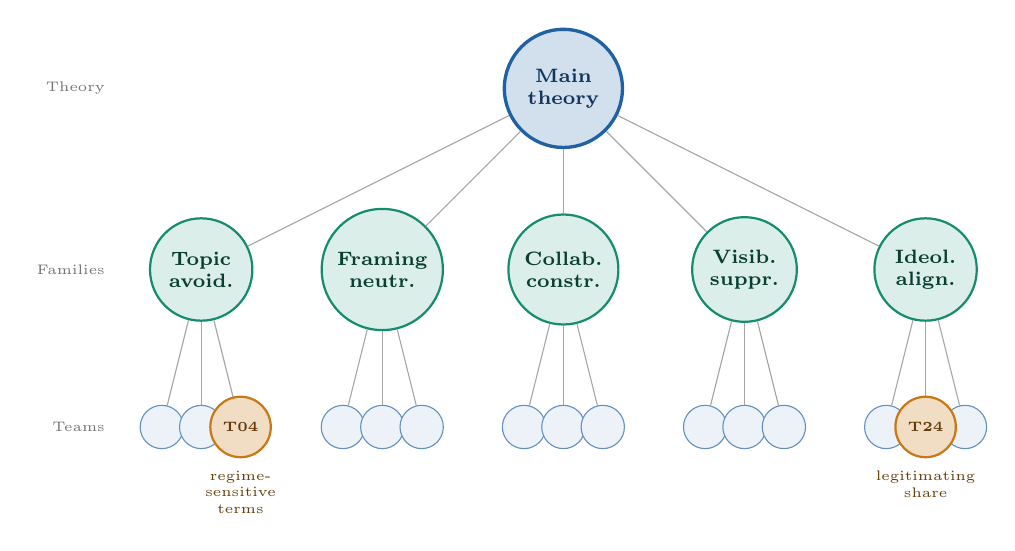
\begin{tikzpicture}[
    every node/.style={font=\scriptsize},
    theory/.style={circle, draw=agentblue, fill=agentblue!20, very thick,
                   minimum size=1.5cm, align=center, text=agentblue!55!black,
                   font=\scriptsize\bfseries},
    fam/.style={circle, draw=milestoneteal, fill=milestoneteal!15, thick,
                minimum size=1.3cm, align=center, text=milestoneteal!45!black,
                font=\scriptsize\bfseries},
    imp/.style={circle, draw=agentblue!70, fill=agentblue!8, minimum size=0.55cm},
    impx/.style={circle, draw=gateamber, fill=gateamber!25, thick,
                 minimum size=0.62cm, font=\tiny\bfseries, text=gateamber!50!black},
    edge/.style={draw=black!35},
  ]
    % row labels (short, to keep width modest)
    \node[anchor=east, text=black!55, font=\tiny] at (0.8,0)    {Theory};
    \node[anchor=east, text=black!55, font=\tiny] at (0.8,-2.3) {Families};
    \node[anchor=east, text=black!55, font=\tiny] at (0.8,-4.3) {Teams};
    % main theory
    \node[theory] (T) at (6.5,0) {Main\\theory};
    % sub-families + plain implications
    \foreach \x/\name/\lab in {%
      1.9/F1/{Topic\\avoid.}, 4.2/F2/{Framing\\neutr.}, 6.5/F3/{Collab.\\constr.},
      8.8/F4/{Visib.\\suppr.}, 11.1/F5/{Ideol.\\align.}} {
        \node[fam] (\name) at (\x,-2.3) {\lab};
        \draw[edge] (T) -- (\name);
        \foreach \dx in {-0.5,0,0.5} {
          \node[imp] (i) at ({\x+\dx},-4.3) {};
          \draw[edge] (\name) -- (i);
        }
      }
    % highlighted worked-example teams (drawn on top of the plain leaves)
    \node[impx] (E1) at (2.4,-4.3) {T04};
    \node[impx] (E2) at (11.1,-4.3) {T24};
    \node[font=\tiny, text=gateamber!50!black, align=center, below=1pt of E1]
      {regime-\\sensitive\\terms};
    \node[font=\tiny, text=gateamber!50!black, align=center, below=1pt of E2]
      {legitimating\\share};
  \end{tikzpicture}}
  \\[0.5em]
  {\footnotesize teams tests offspring implication; the theory is judged on the \emph{distribution} of results.}
\end{frame}

% ===================== 7. Agent Orchestra =====================
\begin{frame}{The Agent Orchestra}
  \small
  \textbf{25 teams}, each a pipeline of AI agents, with a PI gate at every stage
  (human in the loop):
  \vspace{1.2em}

  \centering
  \resizebox{\linewidth}{!}{%
  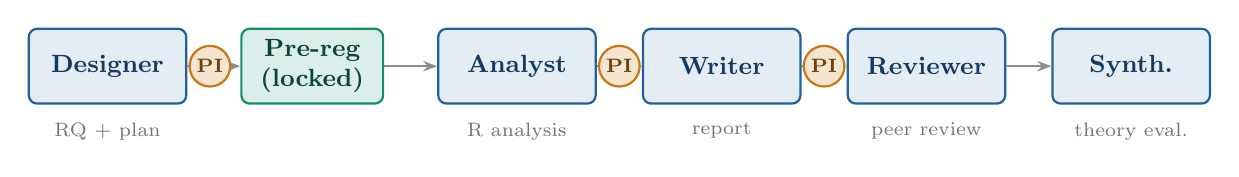
\begin{tikzpicture}[
    agent/.style={rounded corners=3pt, draw=agentblue, fill=agentblue!12, thick,
                  text=agentblue!60!black, font=\small\bfseries,
                  minimum width=2.0cm, minimum height=0.95cm, align=center},
    prereg/.style={rounded corners=3pt, draw=milestoneteal, fill=milestoneteal!15, thick,
                   text=milestoneteal!50!black, font=\small\bfseries,
                   minimum width=1.8cm, minimum height=0.95cm, align=center},
    sub/.style={font=\scriptsize, text=black!55, align=center},
    gate/.style={circle, draw=gateamber, fill=gateamber!20, thick,
                 text=gateamber!55!black, font=\scriptsize\bfseries, inner sep=1.5pt},
    arr/.style={-{Stealth[length=5pt]}, thick, black!45},
  ]
    \node[agent]  (D) at (0,0)    {Designer};
    \node[prereg] (P) at (2.6,0)  {Pre-reg\\(locked)};
    \node[agent]  (A) at (5.2,0)  {Analyst};
    \node[agent]  (W) at (7.8,0)  {Writer};
    \node[agent]  (R) at (10.4,0) {Reviewer};
    \node[agent]  (S) at (13.0,0) {Synth.};
    \foreach \a/\b in {D/P,P/A,A/W,W/R,R/S} \draw[arr] (\a) -- (\b);
    \node[sub, below=3pt of D] {RQ + plan};
    \node[sub, below=3pt of A] {R analysis};
    \node[sub, below=3pt of W] {report};
    \node[sub, below=3pt of R] {peer review};
    \node[sub, below=3pt of S] {theory eval.};
    % PI review gates sitting on the path
    \node[gate] at (1.3,0) {PI};
    \node[gate] at (6.5,0) {PI};
    \node[gate] at (9.1,0) {PI};
  \end{tikzpicture}}
  \\[1.2em]
  {\footnotesize Amber: PI review gate (redesign / revise loop). Hypotheses locked
  before analysis at Git \texttt{960525f}; an emerging method
  \citep{zhu2026hler,gupta2026accelerating}.}
\end{frame}


\begin{frame}{All 25 teams: outcomes and status}
  \hypertarget{ap:teams}{}
  \scriptsize
  \begin{columns}[T]
    \begin{column}{0.5\textwidth}
      \textbf{Topic avoidance}\\[0.2em]
      \begin{tabular}{@{}r@{\;}l@{}}
        01 & PCI (political-content index)\\
        02 & Keyword entropy\\
        03 & Share in sensitive fields\\
        04 & Share w/ regime-sensitive terms\\
        05 & Share critical of own governance$^\dagger$\\
        06 & Semantic diversity (embeddings)$^\dagger$\\
        07 & Share internationally funded\\
      \end{tabular}\\[0.5em]
      \textbf{Framing neutrality}\\[0.2em]
      \begin{tabular}{@{}r@{\;}l@{}}
        08 & Epistemic hedging rate\\
        09 & Normative language rate\\
        10 & Share purely technocratic$^\dagger$\\
        11 & Argumentative stance rate\\
        12 & Share w/ normative conclusion$^\dagger$\\
        13 & Share in domestic journals\\
      \end{tabular}
    \end{column}
    \begin{column}{0.5\textwidth}
      \textbf{Collaboration constraint}\\[0.2em]
      \begin{tabular}{@{}r@{\;}l@{}}
        14 & Mean co-author countries\\
        15 & Share democratic co-authors\\
        16 & Share domestic-only authorship\\
        17 & Mean author count\\
        18 & Mean distinct institutions\\
      \end{tabular}\\[0.5em]
      \textbf{Visibility suppression}\\[0.2em]
      \begin{tabular}{@{}r@{\;}l@{}}
        19 & Log citation ratio\\
        20 & Citation gap by sensitivity\\
        21 & Share ever cited\\
        22 & Citation Gini\\
      \end{tabular}\\[0.5em]
      \textbf{Ideological alignment}\\[0.2em]
      \begin{tabular}{@{}r@{\;}l@{}}
        23 & Share liberal/neutral framing\\
        24 & Share legitimating regime\\
        25 & Share anti-liberal framing\\
      \end{tabular}
    \end{column}
  \end{columns}
  \vspace{0.3em}
  {$^\dagger$ pending (LLM / embeddings); the other 21 are complete.}\hfill\hyperlink{ap:toc}{\beamerreturnbutton{back}}
\end{frame}
% ===================== 8. Data =====================
\begin{frame}{Data: one locked corpus}
  \begin{columns}[T]
    \begin{column}{0.55\textwidth}
      \textbf{Corpus} (Web of Science, SSH)
      \begin{itemize}
        \item \key{2.7M} articles, 167 countries
        \item 1970--2023
        \item 99.98\% matched to V-Dem
      \end{itemize}
    \end{column}
    \begin{column}{0.45\textwidth}
      \textbf{Politics} (V-Dem)
      \begin{itemize}
        \item IV: \texttt{v2x\_libdem}
        \item Controls: log GDPpc, log pop
      \end{itemize}
    \end{column}
  \end{columns}
  \vspace{0.8em}
  \centering Unit: \key{country--year}.
\end{frame}

% ===================== 9. Specification =====================
\begin{frame}{One shared benchmark specification}
  Two-way fixed effects, every team:
  \begin{equation*}
    Y_{it} = \beta\,\texttt{v2x\_libdem}_{it}
      + \gamma_1 \log\text{gdppc}_{it}
      + \gamma_2 \log\text{pop}_{it}
      + \alpha_i + \delta_t + \varepsilon_{it}
  \end{equation*}
  \begin{itemize}
    \item Country + year FE; SE clustered by country.
    \item Secondary: pooled OLS. Robustness: alt.\ measure + binary regime.
    \item \key{Family-wise Bonferroni}, $\alpha = 0.05/k$.
  \end{itemize}
\end{frame}

% ===================== 10. Example 1: Team 04 =====================
\begin{frame}{Example 1, Team 04: topic avoidance}
  \small
  \textbf{Rationale.} Regime-sensitive concepts such as democracy, human rights,
  corruption, and protest are the highest-cost topics under autocracy. A paper's
  most visible labels (title, keywords) are the likeliest site of
  \key{anticipatory avoidance}.
  \vspace{0.4em}
  \begin{itemize}
    \item \textbf{Outcome} \texttt{share\_regime\_sensitive}: share of a
          country-year's articles with $\geq 1$ hit from a regime-sensitive
          dictionary (democracy, rights, corruption, protest, repression, \dots)
          in title, keywords, or abstract.
    \item \textbf{Test:} TWFE on \texttt{v2x\_libdem}; \key{predicted $\beta>0$}
          (more democracy $\rightarrow$ more sensitive terms).
  \end{itemize}
  \vspace{0.3em}
  \begin{block}{Result}
    $\hat\beta = +0.001$ (SE $0.018$), $p = 0.94$, $N = 2{,}803$ country-years.
    \hfill\warn{Indistinguishable from zero.}
  \end{block}
\end{frame}

% ===================== 10b. Example 2: Team 24 =====================
\begin{frame}{Example 2, Team 24: ideological alignment}
  \small
  \textbf{Rationale.} Autocracies do not only suppress dissent; \key{reward}
  scholarship that endorses the regime (state funding, party-controlled outlets,
  promotion criteria). 
  \vspace{0.4em}
  \begin{itemize}
    \item \textbf{Outcome} \texttt{share\_legitimating}: share of abstracts an
          \key{LLM} (Claude Haiku) labels as actively endorsing the political
          system; stratified sample, \textasciitilde141k abstracts classified.
    \item \textbf{Test:} TWFE on \texttt{v2x\_libdem}; \key{predicted $\beta<0$}
          (more autocracy $\rightarrow$ more legitimation).
  \end{itemize}
  \vspace{0.3em}
  \begin{block}{Result}
    $\hat\beta = +0.003$ (SE $0.002$), $p = 0.23$, $N = 3{,}207$ country-years.
    \hfill\warn{Wrong sign, not significant.}
  \end{block}
  \vspace{0.1em}
  \centering{\scriptsize\color{gray} Only 582 of 140{,}879 classified abstracts (0.4\%) coded as legitimating: a rare-event outcome. Completed after the May-27 forest plot was frozen, not shown there.}
\end{frame}

% ===================== 11. Main results =====================
\begin{frame}{Results: coefficients cluster at zero}
  \centering
  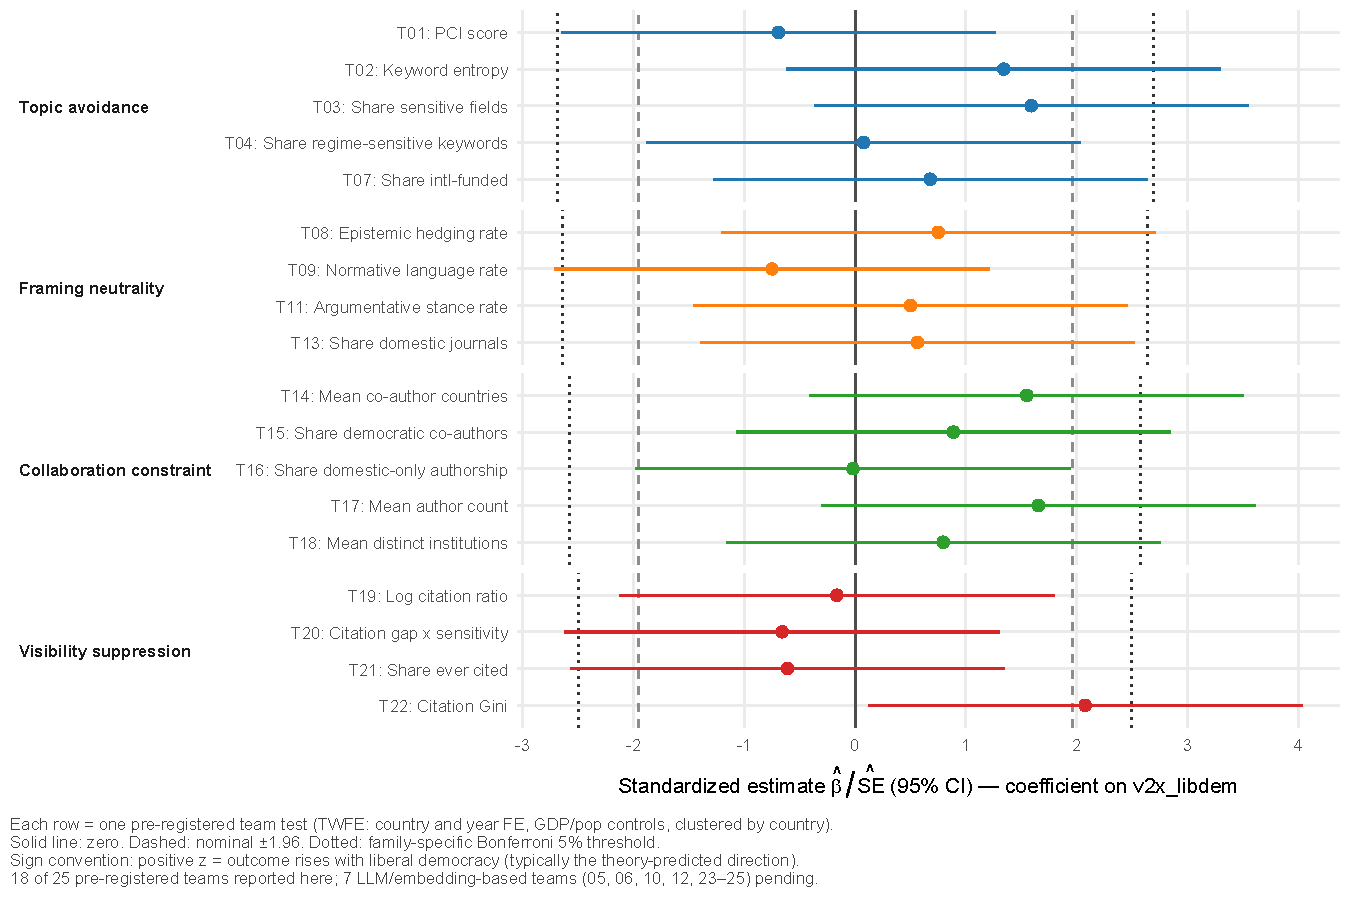
\includegraphics[height=0.74\textheight]{fig_main_coefficients.pdf}\\
  \caveat
\end{frame}

% ===================== 12. Meta-summary =====================
\begin{frame}{Nothing survives correction}
  \centering
  {\small % Auto-generated by scripts/make_meta_summary_table.R - do not edit by hand.
\begin{tabular}{@{}l c c c c c c@{}}
\toprule
 & Registered & Completed & \multicolumn{2}{c}{Sign of $\hat{\beta}$} & Nominal & Bonferroni \\
\cmidrule(lr){4-5}
Sub-family & ($k$) & tests & $>0$ & $<0$ & $p<.05$ & $p<.05$ \\
\midrule
Topic avoidance & 7 & 5 & 4 & 1 & 0 & 0 \\
Framing neutrality & 6 & 4 & 3 & 1 & 0 & 0 \\
Collaboration constraint & 5 & 5 & 4 & 1 & 0 & 0 \\
Visibility suppression & 4 & 4 & 1 & 3 & 1 & 0 \\
\midrule
\textbf{Total} & \textbf{22} & \textbf{18} & \textbf{12} & \textbf{6} & \textbf{1} & \textbf{0} \\
\bottomrule
\end{tabular}
}\\[0.2em]
  {\scriptsize\color{gray} Four corpus-based families (18 teams) shown.}
  \vspace{0.5em}
  \begin{itemize}\small
    \item \key{0 of 18} survive Bonferroni; 1 nominal hit (T22) runs \warn{opposite} to prediction.
    \item Ideological-alignment teams \key{23--25} (now complete) are \key{also null}: $p = 0.13,\,0.23,\,0.16$.
    \item Our two examples land here too: \key{T04} $p=0.94$, \key{T24} $p=0.23$.
  \end{itemize}
\end{frame}

% ===================== 13. Robustness =====================
\begin{frame}{Results}
  \small
  \textbf{Robustness}
  \begin{itemize}
    \item Within-family directions suggestive at best; none significant.
    \item TWFE and pooled OLS \key{agree}: not a fixed-effects artifact.
  \end{itemize}
  \vspace{0.3em}
  \textbf{Power, the leading alternative explanation}
  \begin{itemize}
    \item Large samples (2{,}500--3{,}500 country-years, 150+ countries): well-powered
          for \key{between-country} contrasts.
    \item But TWFE leans on \key{within-country} change in democracy, which is slow and
          rare, so the within estimand is less precisely identified.
    \item Reassurance: confidence intervals sit \key{tight around zero}, ruling out
          large effects, and the cross-sectional (pooled) estimates agree.
    \item \warn{Still open:} small effects, or effects concentrated in specific
          regimes, fields, or periods, cannot be excluded.
  \end{itemize}
\end{frame}

% ===================== 14. Interpretation =====================
\begin{frame}{Results}
  \begin{itemize}
    \item Across 21 dimensions, including LLM-coded \key{ideological alignment},
          \key{little sign} that autocracy bends published content.
    \item \warn{Caveats:}
      \begin{itemize}\small
        \item Observational; content censorship vs.\ \key{venue selection}.
        \item WoS skews English / high-impact; misses domestic outlets.
        \item \key{4 framing teams} (LLM, embeddings) still pending.
      \end{itemize}
  \end{itemize}
  \vspace{0.5em}
  \centering \caveat
\end{frame}

% ===================== 15. Reflection + discussion =====================
\begin{frame}{Summary and discussion}
  \small
  \textbf{Findings.} Across 21 pre-registered tests, including LLM-coded ideological
  alignment, \key{little evidence} that autocracy bends the content of published SSH;
  no coefficient survives correction.
  \vspace{0.3em}

  \textbf{Contribution}
  \begin{itemize}
    \item \textit{Theoretical:} a first broad test of content self-censorship; an
          informative null that shifts the burden of proof.
    \item \textit{Methodological:} an \key{agent-orchestra} many-analysts design that
          scales a multi-implication theory, with pre-registration and human review
          built in.
  \end{itemize}
  \vspace{0.2em}

  \textbf{Limitations.} Observational (content censorship vs.\ venue selection); WoS
  skews English and high-impact, missing domestic outlets; effective power for the
  within estimand is limited; 4 framing teams pending; AI-generated design choices
  raise provenance and refereeing questions.
  \vspace{0.3em}

  \centering\hyperlink{ap:toc}{\beamergotobutton{Appendix / backup slides}}\\[0.3em]
  \color{agentblue}\small tore.wig@stv.uio.no
\end{frame}

% ===================== References =====================
\begin{frame}[allowframebreaks]{References}
  \footnotesize
  \bibliographystyle{apsr}
  \bibliography{autocrat}
\end{frame}

% ===================================================================
% Appendix (separate numbering; clickable index for Q&A)
% ===================================================================
\appendix

\begin{frame}{Appendix: backup slides}
  \hypertarget{ap:toc}{}
  \vspace{0.4em}
  \begin{itemize}\setlength\itemsep{0.5em}
    \item \hyperlink{ap:teams}{\beamergotobutton{All 25 teams: outcomes and status}}
    \item \hyperlink{ap:families}{\beamergotobutton{Five families and Bonferroni thresholds}}
    \item \hyperlink{ap:spec}{\beamergotobutton{Estimation: specification and robustness}}
    \item \hyperlink{ap:data}{\beamergotobutton{Data and corpus construction}}
    \item \hyperlink{ap:llm}{\beamergotobutton{LLM classification (ideological alignment)}}
    \item \hyperlink{ap:prereg}{\beamergotobutton{Pre-registration, gates, pending teams}}
  \end{itemize}
\end{frame}


\begin{frame}{Five families and Bonferroni thresholds}
  \hypertarget{ap:families}{}
  \small
  \centering
  \begin{tabular}{llcc}
    \toprule
    Sub-family & Teams & $k$ & Adjusted $\alpha$ ($0.05/k$)\\
    \midrule
    Topic avoidance          & 01--07 & 7 & $p < 0.0071$\\
    Framing neutrality       & 08--13 & 6 & $p < 0.0083$\\
    Collaboration constraint & 14--18 & 5 & $p < 0.0100$\\
    Visibility suppression   & 19--22 & 4 & $p < 0.0125$\\
    Ideological alignment    & 23--25 & 3 & $p < 0.0167$\\
    \midrule
    \textbf{Total}           & 01--25 & \textbf{25} & \\
    \bottomrule
  \end{tabular}\\[0.8em]
  {\small Bonferroni applied within each family; predicted signs are in each team's preregistration.}
  \vfill
  \hfill\hyperlink{ap:toc}{\beamerreturnbutton{back}}
\end{frame}

\begin{frame}{Estimation: specification and robustness}
  \hypertarget{ap:spec}{}
  \small
  \textbf{Primary (TWFE), every team:}
  \begin{equation*}
    Y_{it} = \beta\,\texttt{v2x\_libdem}_{it} + \gamma_1 \log\text{gdppc}_{it}
      + \gamma_2 \log\text{pop}_{it} + \alpha_i + \delta_t + \varepsilon_{it}
  \end{equation*}
  \begin{itemize}
    \item $\alpha_i$ country FE, $\delta_t$ year FE; SE clustered by country.
    \item \textbf{Secondary:} pooled OLS, year FE only (cross-sectional pattern).
    \item \textbf{RC1:} alternative operationalization or sample restriction.
    \item \textbf{RC2:} replace \texttt{v2x\_libdem} with \texttt{lied\_binary}.
    \item Unit: country-year; minimum 10 articles per country-year (most teams).
  \end{itemize}
  \vfill
  \hfill\hyperlink{ap:toc}{\beamerreturnbutton{back}}
\end{frame}

\begin{frame}{Data and corpus construction}
  \hypertarget{ap:data}{}
  \small
  \begin{itemize}
    \item Source: Web of Science, all SSH subject categories.
    \item 3{,}189{,}557 article-country rows; 2{,}709{,}224 unique articles.
    \item Years 1970--2023; 167 countries; 99.98\% matched to V-Dem by ISO3.
    \item De-duplication and V-Dem merge: \texttt{scripts/00\_prepare\_data.R}.
    \item IV \texttt{v2x\_libdem} (0--1); controls log GDP per capita, log population.
    \item Robustness IV \texttt{lied\_binary}; regime type \texttt{v2x\_regime} (0--3).
    \item Corpus locked before any analysis.
  \end{itemize}
  \vfill
  \hfill\hyperlink{ap:toc}{\beamerreturnbutton{back}}
\end{frame}

\begin{frame}{LLM classification (ideological alignment)}
  \hypertarget{ap:llm}{}
  \small
  Teams 23--25 code abstracts with an LLM (Claude Haiku). Example, Team 24:
  \vspace{0.3em}
  \begin{itemize}
    \item \textbf{Binary label.} LEGITIMATING: the abstract explicitly endorses or
          validates the political system, state authority, ruling party, or leadership
          as effective, beneficial, or necessary. NON-LEGITIMATING: everything else
          (default when in doubt).
    \item \textbf{Sample.} Stratified by country $\times$ regime $\times$ decade; up to
          10 abstracts per stratum; abstracts of $\geq 50$ characters; fixed seed.
    \item \textbf{Aggregation.} Share LEGITIMATING per country-year, then TWFE as usual.
    \item \textbf{Scale.} About 141k abstracts classified for Team 24.
  \end{itemize}
  \vfill
  \hfill\hyperlink{ap:toc}{\beamerreturnbutton{back}}
\end{frame}

\begin{frame}{Pre-registration, gates, pending teams}
  \hypertarget{ap:prereg}{}
  \small
  \textbf{Pre-registration.} All 25 hypotheses, predicted signs, primary specifications,
  robustness checks, and Bonferroni families were locked at Git commit \texttt{960525f}
  (6 May 2026), before any analyst session ran.
  \vspace{0.3em}
  \begin{itemize}
    \item \textbf{Gates.} PI review at design (B), results (D), and report (G); revision
          loops allowed for implementation only, not for outcomes.
    \item \textbf{Complete (21):} all corpus-based teams plus ideological alignment (23--25).
    \item \textbf{Pending (4):} 05 (critical governance, LLM), 06 (semantic diversity,
          embeddings), 10 (technocratic share, LLM), 12 (normative conclusion, LLM).
  \end{itemize}
  \vfill
  \hfill\hyperlink{ap:toc}{\beamerreturnbutton{back}}
\end{frame}

\end{document}
